\documentclass[../notes.tex]{subfiles}

\begin{document}

\section{CUDA}

\subsection{Key Concepts}

\subsubsection{Data Parallelism}
GPU is traditionally used for rendering graphics. For example, per-pixel lighting is a highly parallel, and data-intensive task and a GPU is perfect for the job. We can map each pixel with a thread and they all can be processed in O(1) constant time.

Image processing and computer graphics are not the only areas in which we harness data parallelism to our advantage. Many high-performance algebra libraries today such as CU-BLAS harness the processing power of the modern GPU to perform data intensive algebra operations.

\subsubsection{Program Structure of CUDA}
A typical CUDA program has code intended both for the GPU and the CPU. By default, a traditional C program is a CUDA program with only the host code. The CPU is referred to as the host, and the GPU is referred to as the device. Whereas the host code can be compiled by a traditional C compiler as the GCC, the device code needs a special compiler to understand the api functions that are used. For Nvidia GPUs, the compiler is called the NVCC (Nvidia C Compiler).

The device code runs on the GPU, and the host code runs on the CPU. The NVCC processes a CUDA program, and separates the host code from the device code. To accomplish this, special CUDA keywords are looked for. The code intended to run of the GPU (device code) is marked with special CUDA keywords for labelling data-parallel functions, called ‘Kernels’. The device code is further compiled by the NVCC and executed on the GPU.

\subsubsection{Execution of a CUDA C Program}
While writing a CUDA program, the programmer has explicit control on the number of threads that he wants to launch. These threads collectively form a three-dimensional grid (threads are packed into blocks, and blocks are packed into grids). Each thread is given a unique identifier, which can be used to identify what data it is to be acted upon.

\textbf{Device Global Memory and Data Transfer}
As has been explained in the previous chapter, a typical GPU comes with its own global memory (DRAM- Dynamic Random Access Memory). We call this memory the device memory.

To execute a kernel on the GPU, the programmer needs to allocate separate memory on the GPU by writing code. The CUDA API provides specific functions for accomplishing this. Here is the flow sequence:

\begin{enumerate}
  \item After allocating memory on the device, data has to be transferred from the host memory to the device memory.
  \item After the kernel is executed on the device, the result has to be transferred back from the device memory to the host memory.
  \item The allocated memory on the device has to be freed-up. The host can access the device memory and transfer data to and from it, but not the other way round.
\end{enumerate}

CUDA provides API functions to accomplish all these steps.

\newpage

\subsection{Key Worlds and Thread Organization}
\begin{tabular}{ |c|c|c| } 
  \hline
   & EXECUTED ON THE & CALLABLE FROM \\
  \hline
  \_\_device\_\_ float function() & GPU (device) & GPU (device) \\
  \hline
  \_\_global\_\_ void function() & GPU (device) & CPU (host) and GPU (device) \\ 
  \hline
  \_\_host\_\_ float function() & CPU (host) & CPU (host) \\ 
  \hline
\end{tabular}

\textbf{Functions}
\begin{itemize}
\item cudaMalloc() - This method is used to allocate memory on the host. in two parameters, the address of a pointer to the allocated object, and the size of the allocated object in terms of bytes.
\item cudaMemcpy() - This API function is used for memory data transfer. It requires four parameters as input: Pointer to the destination, pointer to the source, amount of data to be copied (in bytes), and the direction of transfer.
\item cudaFree() - This method is used to release objects from device memory. It takes in the pointer to the freed object as parameter.
\end{itemize}

\textbf{CUDA Thread Organization}

Threads in a grid execute the same kernel function. They have specific coordinates to distinguish themselves from each other and identify the relevant portion of data to process. In CUDA, they are organized in a two-level hierarchy: a grid comprises blocks (can be accessed using the \textbf{blockIdx}), and each block comprises threads (can be accessed using the \textbf{threadIdx}). Note that blockIdx and threadIdx are built-in CUDA variables that are only accessible from inside the kernel.

In a similar fashion, CUDA also has gridDim and blockDim variables that are also built-in. They return the dimensions of the grid and block along a particular axis respectively.

\subsection{Threads}
\subsubsection{Resources Assignment to Blocks}
Execution resources are assigned to threads per block. Resources are organized into Streaming Multiprocessors (SM). Multiple blocks of threads can be assigned to a single SM.

Thus, the number of threads that can run parallel on a CUDA device is simply the number of SM multiplied by the maximum number of threads each SM can support.

\subsubsection{Synchronization between Threads}
The CUDA API has a method, \textbf{\_\_syncthreads()} to synchronize threads. When the method is encountered in the kernel, all threads in a block will be blocked at the calling location until each of them reaches the location. It ensure phase synchronization. That is, all the threads of a block will now start executing their next phase only after they have finished the previous one.

If a \_\_syncthreads statement, is present in the kernel, it must be executed by all threads of a block. If it is present inside an if statement, then either all the threads in the block go through the if statement, or none of them does. As all the threads of a block have to execute the sync method call, if threads took different paths, then they will be blocked forever. It is the duty of the programmer to be wary of such conditions that may arise.

\subsubsection{Thread Scheduling}
After a block of threads is assigned to a SM, it is divided into sets of 32 threads, each called a warp. Here are some important properties of warps:

\begin{itemize}
\item A warp is a unit of thread scheduling in SMs. That is, the granularity of thread scheduling is a warp. A block is divided into warps for scheduling purposes.
\item A SM is composed of many SPs (Streaming Processors). These are the actual CUDA cores. Normally, the number of CUDA cores in a SM is less than the total number of threads that are assigned to it. Thus the need for scheduling.
\item While a warp is waiting for the results of a previously executed long-latency operation (like data fetch from the RAM), a different warp that is not waiting and is ready to be assigned is selected for execution. This means that threads are always scheduled in a group.
\item If more than one warps are on the ready queue, then some priority mechanism can be used for assignment.
\item A warp consists of threads with consecutive threadIdx.x values. For example, threads of the first warp will have threads ids b/w 0 to 31. Threads of the second warp will have thread ids from 32-63.
\item All threads in a warp follow the SIMD (Single Instruction, Multiple Data) model. In SIMD, each thread is executing the same instruction of a kernel at any given time. But the data is always different.
\end{itemize}

\textbf{Latency Tolerance}
A lot of processor time goes waste if while a warp is waiting, another warp is not scheduled. This method of utilizing in the latency time of operations with work from other warps is called latency tolerance.

\subsection{Performace Consideration}
CGMA stands for ‘Compute to Global Memory Access’ ratio, and the higher it is, the better the kernel performs. Programmers should aim to increase this ratio as much as it possible.

Memory is often a bottleneck to achieving high performance in CUDA programs. No matter how fast the DRAM is, it cannot supply data at the rate at which the cores can consume it.

\newpage

\subsection{Memory}
Apart from the device DRAM, CUDA supports several additional types of memory that can be used to increase the CGMA ratio for a kernel. We know that accessing the DRAM is slow and expensive. To overcome this problem, several low-capacity, high-bandwidth memories, both on-chip and off-chip are present on a CUDA GPU. If some data is used frequently, then CUDA caches it in one of the low-level memories. Thus, the processor does not need to access the DRAM every time. The following figure illustrates the memory architecture supported by CUDA and typically found on Nvidia cards.

\textbf{Device Code}
\begin{itemize}
\item R/W per-thread registers
\item R/W per-thread local memory
\item R/W per-block shared memory
\item R/W per-grid global memory
\item Read only per-grid const memory
\end{itemize}

\begin{figure}[h]
  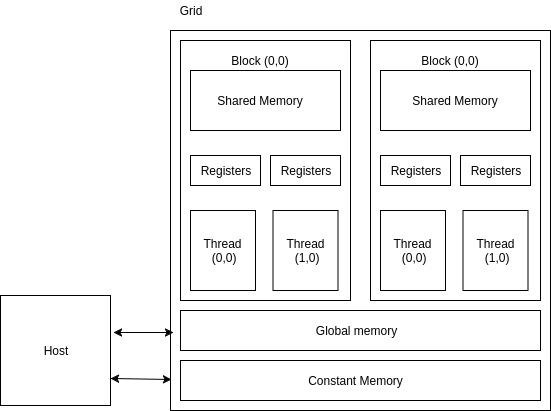
\includegraphics[width=12cm]{device_code}
\end{figure}

\textbf{Host code}

This helps in transferring data to/from per grid global and constant memories. 

The global memory is a high-latency memory (the slowest in the figure). To increase the arithmetic intensity of our kernel, we want to reduce as many accesses to the global memory as possible. One thing to note about global memory is that there is no limitation on what threads may access it. All the threads of any block can access it. There are no restrictions, like there are in the case of shared memory or registers.

The constant memory can be written into and read by the host. It is used for storing data that will not change over the course of kernel execution. It supports short-latency, high-bandwidth, read-only access by the device when all threads simultaneously access the same location. The constant memory is cached. For all threads of a half warp, reading from the constant cache, as long as all threads read the same address, is no slower than reading from a register. However, if threads of the half-warp access different memory locations, the access time scales linearly with the number of different addresses read by all threads within the half-warp.

\subsubsection{How does constant memory work?}
The following are the steps that are followed when a constant memory access is done by a warp:

\begin{itemize}
\item The request is broken into two parts, one for each half-wrap. That is, two constant memory accesses will take place for a single request.
\item The request for each half-warp is split into as many discrete requests as there are different memory addresses in the initial request, decreasing the throughput by a factor equal to the number of separate requests. The cost increases linearly. If there is just one memory address that is accessed, then the access is as fast as it is from a register.
\item If there is a cache hit, then the resulting data is serviced at the bandwidth of the cache.
\item In case of a cache miss, the resulting data is serviced at the bandwidth of the DRAM.
\end{itemize}

The \_\_constant\_\_ keyword can be used to store a variable in constant memory. They are always declared as global variables.

Registers and shared-memory are on-chip memories. Variables that are stored in these memories are accessed at a very high speed in a highly parallel manner. A thread is allocated a set of registers, and it cannot access registers that are not parts of that set. A kernel generally stores frequently used variables that are private to each thread in registers. The cost of accessing variables from registers is less than that required to access variables from the global memory.

\subsubsection{Shared Memory}
All threads of a block can access its shared memory. Shared memory can be used for inter-thread communication. Each block has its own shared-memory. Just like registers, shared memory is also on-chip, but they differ significantly in functionality and the respective access cost.

While accessing data from the shared memory, the processor needs to do a memory load operation, just like accessing data from the global memory. This makes them slower than registers, in which the LOAD operation is not required. Since it resides on-chip, shared memory has shorter latency and higher bandwidth than global memory.

\subsubsection{Variable Lifetime}
Lifetime of a variable tells the portion of the program’s execution duration when it is available for use. If a variable’s lifetime is within the kernel, then it will be available for use only by the kernel code. An important point to note here is that multiple invocations of the kernel do not maintain the value of the variable across them.

\textbf{Automatic Variables}

Automatic variables are those variables for which a copy exists for each thread. In the matrix multiplication example, row and col are automatic variables. A private copy of row and col exists for each thread, and once the thread finishes execution, its automatic variables are destroyed.

The following table summarizes the lifetime, scope and memory of different types of CUDA variables:

\begin{tabular}{ |c|c|c|c| } 
  \hline
  Variable declaration & Memory & Scope & Lifetime \\
  \hline
  Automatic variables other than arrays & Register & Thread & Kernel \\
  \hline
  Automatic array variables & Local & Thread & Kernel\\
  \hline
  \_\_device\_\_ \_\_shared\_\_ int sharedVar & Shared & Block & Kernel \\
  \hline
  \_\_device\_\_ int globalVar & Global & Grid & Application \\ 
  \hline
  \_\_device\_\_ \_\_constant\_\_ int constVar & Constant & Grid & Application \\ 
  \hline
\end{tabular}

Constant variables are stored in the global memory (constant memory), but are cached for efficient access. They can be accessed in a highly-parallel manner at high-speeds. As their lifetime equals the lifetime of the application, and they are visible to all the threads, declaration of constant variables must be done outside any function.

\subsubsection{Memory as a Bottleneck}
Although shared memory and registers are high-speed memories with huge bandwidth, they are available in limited amounts in a CUDA device. A programmer should be careful not to overuse these limited resources. The limited amount of these resources also caps the number of threads that can actually execute in parallel in a SM for a given application. The more resources a thread requires, the less the number of threads that can simultaneously reside in the SM. It is simply because there is a dearth of resources.

Shared memory usage can also limit the number of threads assigned to each SM. Suppose that a CUDA GPU has 16k/SM of shared memory. Suppose that each SM can support upto 8 blocks. To reach the maximum, each block must use no more than 2k of shared memory. If each block uses 5k of shared memory, then no more than 3 blocks can live in a SM.

\subsection{Memory Considerations}
Memory coalescing is one of the most important things that are taken into account while writing CUDA applications. Coalesced memory accesses improve the performance of your applications drastically.

Data bits in DRAM cells are stored in very weak capacitors that hold charge to distinguish between 1 and 0. A charge capacitor contains 1, and it shares its charge with a sensor that determines if it was sufficiently charged to represent a 1. This process is slow, and accessing a bit like this would be very inefficient. Instead, what actually happens is that many consecutive cells transfer their charges in parallel to increase bandwidth. There are multiple sensors present that detect charges on these cell in parallel. Whenever a location is accessed in the DRAM, data at locations adjacent to it are also accessed and supplied. Now, if that data were actually needed, then it is used and bandwidth is saved. Otherwise, it goes to waste.

We already know that threads in a warp execute the same instruction at any point in time. Let the instruction be LOAD (LD). If it so happens that the threads are accessing consecutive memory locations in the DRAM, then their individual requests can be coalesced into one. This is detected by the hardware dynamically, and saves a lot of DRAM bandwidth. When all threads of a warp access consecutive memory locations, it is the most optimal access pattern. For example, if thread 0 of the warp accesses location 0 of the DRAM, thread 1 accesses location 1, and so on, their requests will be merged into one. Such access patterns enable the DRAM to supply data close to their peak bandwidth.

\subsection{Reducing Global Memory Traffic}
Resources in SM are dynamically partitioned and assigned to threads to support their execution. The number of resources in SM are limited, and the higher the demands of a thread, the lower the number of threads that can actually run parallel inside the SM.

The current generation of CUDA devices support up to 1536 thread slots. Each SM can support no more than 1536 threads that can run in parallel. It has to be remembered that there is no capping on the number of thread blocks that can occupy a SM. They can be as many as would keep the total number of threads less than or equal to 1536 per SM. For example, there may be 3 blocks of 512 threads each, or 6 blocks of 256 threads each, or 12 blocks of 128 threads each.

\subsubsection{Reducing Traffic to the Global Memory Using Tiles}
\subsubsection{Tiled Matrix-Matrix Multiplication}

\subsection{Caches}
Architecture designers used small memories made up of SRAM that lay very close to the processor. These memories are called caches, and they can transmit data to the processor at a much higher rate than DRAM. But they are typically small in size. The modern GPU contains three levels of caching – L1, L2 and L3. The L1 cache has higher bandwidth compared to other L2 and L3 caches. As we go farther from the cores, the size of the memory increases and its bandwidth decreases.

Caches have been around because of the following attributes of most of the computer programs:
\begin{itemize}
\item Temporal locality - Programs tend to use data that they have used recently.
\item Spatial locality - Programs tend to access data residing in addresses similar to recently referenced data.
\end{itemize}

Computer programs have something called as a working set. The working set of a program can be defined as the set of data a program needs during a certain interval of time to do a certain task. If the working set can be stored in a cache, then the program won’t have to go to the higher levels of memory to fetch data.

\subsection{Cache Implementation}
One important thing to note is that caches are completely transparent to the operating system, which means the OS does not have any knowledge if the working set of the program is cached. Because kernel calls are very expensive, and if the OS takes into account the presence of caches, the increase in the time required to generate an address would offset any benefits that caches offer.

Since the CPU still generates the same address, we need to map the generated addresses with the cached address to access it. In caches, data are stored in blocks (also called lines). A block is a unit of replacement - that is, if some new data comes to be cached, a block of data would be evicted. There are several types of caches:

\textbf{Direct mapped cache}

This is a simple cache. Blocks of the RAM map the cache size to their respective address module. On a conflict, it evicts a block. The advantage is that it is really simple to implement, and is very fast. The downside is that due to a simple hash function, many conflicts may arise.

\textbf{Associative cache}
In associative caches, we have a set of associated blocks in them. Now, blocks from the RAM may map to any block in a particular set. They are of many types – 2-way, 4-way, 8-way. If the cache is an n-way associative cache, then it can eliminate conflicts; if at max n blocks in the RAM map to the same block in the cache concurrently. These types of caches are hard to implement than direct mapped caches. The access time is slower and the hardware required is expensive. Their advantage is that they can eliminate conflicts completely.

\textbf{Fully associative cache}
In these caches, any block of the RAM can block to any block in the cache. Conflicts are eliminated completely, and it is the most expensive to implement.

\subsection{Cache Misses}
Caches have 4 kinds of misses:

\textbf{Compulsory misses:}
When the cache is empty initially, and data come to it for caching. There is not much that can be done about it. One thing that can be done is prefetching. That is, while you are fetching some data from the RAM into the cache, also ensure that the data you will be requiring next are present in the same block. This would prevent a cache miss the next time.

\textbf{Conflict misses:}
These type of misses happen when data need to be fetched again from the RAM as another block mapped to the same cache line and the data were evicted. It should be noted here that fully-associative caches have no conflict misses, whereas direct mapped caches have the most conflict misses.

\textbf{Capacity misses}
These misses occur when the working set of the program is larger than the size of the cache itself. It is simply because some blocks of data are discarded as they cannot fit into the cache. The solution is that the working set of a program should be made smaller.

\textbf{Coherence misses}
These happen in distributed caches where there is in-consistent data in the same distributed cache.

\end{document}
